\documentclass[czech]{beamer}

\usepackage{babel}
\usepackage[utf8]{inputenc}
%\usepackage[unicode]{hyperref}
\usepackage{default}
\usepackage{times}  % fonts are up to you
\usepackage{graphicx}
\usepackage{listings}
\usepackage{courier}

\mode<presentation> {
  \usetheme{Boadilla}
}

\title{Angular JS}
\institute[CVUT FIT]{Fakulta informacních technologí}
\author{Lubomír Čuhel}
\institute[FIT]

\begin{document}
    \begin{frame}
        \titlepage
    \end{frame}

    \begin{frame}
        \frametitle{Osnova}
        \tableofcontents
    \end{frame}

    \section{Co je to Angular JS?}
    \begin{frame}
        \begin{block}{Co je to Angular JS?}
	        Angular JS je JavaScriptový open-source framework MVC architektury, dnes vyvýjený Googlem. Vytváří jednostránkové aplikace, které běží na straně klienta.
        \end{block}
        \begin{block}{Hlavní přednosti}
            \begin{itemize}
                \item MVC architektura
                \item Two-way-binding
                \item HTML5 + Directives šablony
                \item Testovatelnost
                \item Dependency injection
                \item Rychlost
            \end{itemize}        
        \end{block}
    \end{frame}

    \section{Jak začít?}
    \begin{frame}
        \begin{block}{Jak začít?}
            \begin{itemize}
                \item Stránky projektu - \href{http://angularjs.org/}{www.angularjs.org}
                \item Dokumentace  - \href{http://docs.angularjs.org/}{docs.angularjs.org}
                \item Angular-seed app - \href{http://www.github.com/angular/angular-seed}{www.github.com/angular/angular-seed}
            \end{itemize}
            
        \end{block}
        \begin{block}{Doporučuji tutoriály}
            \begin{itemize}
                \item PhoneCat - \href{http://docs.angularjs.org/tutorial}{docs.angularjs.org/tutorial}
                \item \href{http://youtu.be/HCR7i5F5L8c}{Design Decisions in AngularJS (video)}
                \item \href{http://youtu.be/i9MHigUZKEM}{AngularJS Fundamentals In 60-ish Minutes (video)}
                \item \href{http://campus.codeschool.com/courses/shaping-up-with-angular-js/intro}{Shaping up with angular (kurz)}
            \end{itemize}        
        \end{block}
    \end{frame}

    \section{Two-way data binding}
    \begin{frame}
        \begin{block}{Two-way data binding}
            Jedná se o automatickou synchronizaci dat mezi view a modelem.
        \end{block}
        \begin{figure}[ht]
            \centering
            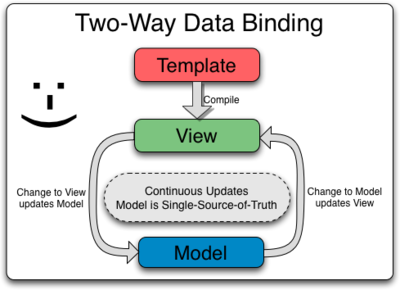
\includegraphics[width=60mm]{two-way-data-binding.png}
            \caption{Two-way data binding\cite{binding}}
            \label{obr:binding}
        \end{figure}

        \begin{thebibliography}{1}
            \bibitem{binding} 
            \small [1] Angular JS [online]. 2013-02-20 [cit. 2014-06-11]. Dostupné z: http://docs.angularjs.org/guide/dev\_guide.templates.databinding
        \end{thebibliography}
    \end{frame}

    \begin{frame}
        \begin{figure}           
            \parbox{.80\linewidth}{\lstinputlisting[language=HTML, frame=single, numbers=left, numbersep=5pt, basicstyle=\footnotesize\ttfamily]{binding.html}}            
        \end{figure}
    \end{frame}
  
    \section{Otázky}
    \begin{frame}
        \centering {Dotazy?}
    \end{frame}
\end{document}
